\documentclass[12pt]{article}
\usepackage{graphicx}
\usepackage{geometry}
\usepackage{hyperref}
\usepackage{enumitem}
\usepackage{titlesec}

\geometry{letterpaper, margin=1.5in}

\titleformat{\section}{\normalfont\fontsize{12}{15}\bfseries}{\thesection}{1em}{}
\titleformat{\subsection}{\normalfont\fontsize{12}{15}\bfseries}{\thesubsection}{1em}{}

\begin{document}

\begin{titlepage}
    \centering
    \includegraphics[width=0.5\textwidth]{fast.png}\par\vspace{0.9cm}
    
    {\scshape\large {{Computer Networks project}} \par}
    \vspace{0.1cm}
    { {\Huge {Fast Nuces University Campus Architecture\\}} \par}
      \vspace{1.5cm}
    { Group Members: \par}
    \vspace{0.1cm}
    {\large Qasim Hasan 21K-3210 \par}
    {\large Talha Shahid 21K-3355 \par}
    {\large Shahmir Raza 21K-3158 \par}
    {\ \par}
    \vspace{1.0cm}
    {\large Instructor: \par}
    \vspace{0.1cm}
    {\large Sir Shaheer Ahmed \par}
    \vspace{1cm}
    {\large Section: \par}
    \vspace{0.1cm}
    {\large BCS-6J \par}
\end{titlepage}

\tableofcontents
\thispagestyle{empty}

\newpage

\section{Introduction}
FAST National University of Computing and Emerging Sciences (FAST-NUCES) is a prestigious institution with two campuses located 30 kilometers apart. The university comprises four faculties: Business, Engineering/Computing, and Electrical. Each faculty is equipped with modern computing facilities, including PCs for both staff and students. The architecture of both campuses and their connection between them includes the use of routing for the email server hosted by a third-party company. Inside the campus buildings, switches are used for both wired and wireless networks.

\section{Campus Network Design Topology}
\begin{figure}[h]
    \centering
    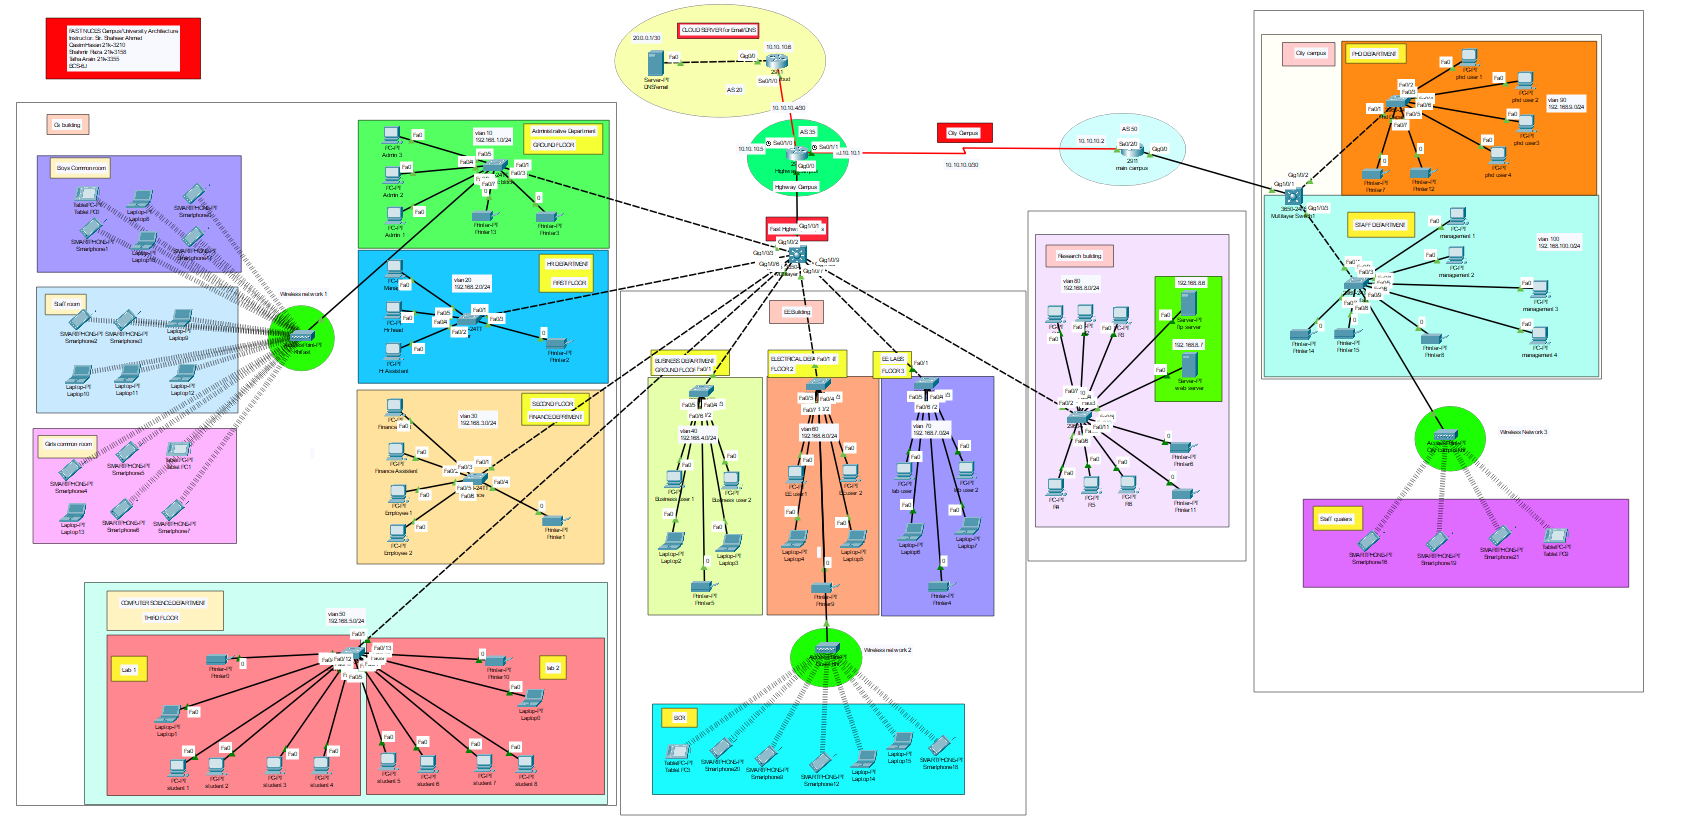
\includegraphics[width=0.8\textwidth]{topo_CN.PNG} 
    \caption{Campus Network Design Topology}
\end{figure}

\section{Main Campus Infrastructure}
\subsection{CS Building}
This building houses the Faculty of Computer Science and has four departments. 
\begin{itemize}[label=--,leftmargin=*,parsep=0pt,itemsep=4pt]
    \item \textbf{Ground Floor}: Administrative department (VLAN 10) and boys' common room (VLAN 10).
    \item \textbf{First Floor}: HR department (VLAN 20) and staff room (VLAN 10).
    \item \textbf{Second Floor}: Finance department (VLAN 30) and girls' common room (VLAN 10).
    \item \textbf{Third Floor}: Computer Science department (VLAN 50) with two labs, Lab1 and Lab2.
\end{itemize}

\subsection{EE Building}
The Faculty of Engineering and Computing is located here.
\begin{itemize}[label=--,leftmargin=*,parsep=0pt,itemsep=4pt]
    \item \textbf{Ground Floor}: Business department (VLAN 40).
    \item \textbf{First Floor}: Electrical department (VLAN 60) and a BCR (VLAN 60).
    \item \textbf{Second Floor}: EE labs (VLAN 70).
\end{itemize}

\subsection{Research Building}
This building is dedicated to research activities and also houses FTP and HTTP web servers.

\section{City Campus}
The City Campus is a smaller campus with separate floors dedicated to different departments.

\begin{itemize}[label=--,leftmargin=*,parsep=0pt,itemsep=4pt]
    \item \textbf{Ground Floor}: Staff department with staff quarters (VLAN 100).
    \item \textbf{First Floor}: PhD department (VLAN 90).
\end{itemize}

\section{Network Technologies Implemented}
\subsection{Routing Algorithms}
\begin{enumerate}
    \item \textbf{BGP (Border Gateway Protocol)}: BGP is used for routing between autonomous systems on the Internet. It ensures reliable routing and allows for policy-based routing decisions.
    \item \textbf{RIPv2 (Routing Information Protocol Version 2)}: RIPv2 is used for dynamic routing within the internal network. It provides a simple and efficient way to exchange routing information.
    \item \textbf{EIGRP (Enhanced Interior Gateway Routing Protocol)}: EIGRP is a Cisco proprietary routing protocol that provides faster convergence and better scalability than traditional routing protocols.
    \item \textbf{Static Routing}: Static routing is configured for external servers, providing a manually defined path for data packets to follow.
    \item \textbf{OSPF (Open Shortest Path First)}: OSPF is used for dynamic routing within the internal network. It is widely used due to its efficiency and scalability.
\end{enumerate}

\subsection{Hierarchical Network Design}
The network is structured hierarchically, with distinct layers for core, distribution, and access. This design facilitates efficient traffic flow and simplifies network management.

\subsection{VLANs and IP Addressing}
VLANs are utilized to segment the network logically, while subnetting optimizes IP address allocation and network efficiency.

\subsection{Inter-VLAN Routing}
Inter-VLAN routing enables communication between devices in different VLANs, ensuring seamless connectivity across the network.

\subsection{DHCP Server Configuration}
DHCP simplifies IP address management by dynamically assigning addresses to devices as they connect to the network, eliminating the need for manual IP address configuration.

\subsection{Email and DNS Servers}
An email server and DNS server are implemented to enable anyone to email using the university domain. The DNS server resolves domain names to IP addresses, ensuring reliable access to online resources.

\subsection{Main Campus Web Server and FTP Server}
The main campus hosts a web server and FTP server, accessible only to users under the architectural network. This ensures secure access to web and file transfer services within the network.

\section{Testing the Campuses Network Architecture}
\begin{itemize}[label=--,leftmargin=*,parsep=0pt,itemsep=4pt]
    \item The network topology is thoroughly tested and verified to ensure that all connectivity requirements are met. This includes testing network communication between devices and verifying the functionality of DHCP, routing protocols, and security measures.
    \item Manual testing is performed by sending data to and from different subnets to verify the integrity of the network.
\end{itemize}

\section{Configuration Commands}

\subsection{Highway campus Configuration}
\begin{verbatim}
enable
configure terminal

int gig0/0
no sh

int se0/1/0
no sh

int se0/1/1
no sh

do wr
exit

\end{verbatim}

\subsection{Highway campus Serial Configuration}
\begin{verbatim}
en
conf t
int se0/1/1
clock rate 64000
int se0/1/0
clock rate 64000
do wr
exit
\end{verbatim}

\subsection{Highway campus IP Configuration}
\begin{verbatim}
en
conf t

int se0/1/1
ip address 10.10.10.1 255.255.255.252 
exit
do wr

int se0/1/0
ip address 10.10.10.5 255.255.255.252 
exit
do wr

\end{verbatim}

\subsection{Cloud server router Configuration}
\begin{verbatim}
enable
configure terminal

int gig0/0
no sh

int se0/1/0
no sh

do wr
exit
\end{verbatim}

\subsection{Cloud server IP Configuration}
\begin{verbatim}
en
conf t

int se0/1/0
ip address 10.10.10.6 255.255.255.252 
exit
do wr

int gig0/0
ip address 20.0.0.1 255.255.255.252 
exit
do wr
\end{verbatim}

\subsection{City campus router Configuration}
\begin{verbatim}
enable
configure terminal

int gig0/0
no sh

int se0/2/0
no sh

do wr
exit
\end{verbatim}

\subsection{City campus IP Configuration}
\begin{verbatim}
en
conf t
int se0/2/0
ip address 10.10.10.2 255.255.255.252 
exit
do wr
\end{verbatim}

\section{Configuring Access Ports for VLANs layer 2 switches}
\subsection{Administrative Department}
\begin{verbatim}

en 
configure terminal
interface range fa0/1-24
switchport mode access
switchport access vlan 10
do wr
exit
\end{verbatim}

\subsection{HR Department}
\begin{verbatim}

en 
configure terminal
interface range fa0/1-24
switchport mode access
switchport access vlan 20
do wr
exit
\end{verbatim}

\subsection{Finance Department}
\begin{verbatim}

en 
configure terminal
interface range fa0/1-24
switchport mode access
switchport access vlan 30
do wr
exit
\end{verbatim}

\subsection{Business Department}
\begin{verbatim}

en 
configure terminal
interface range fa0/1-24
switchport mode access
switchport access vlan 40
do wr
exit
\end{verbatim}

\subsection{Computer Science Department}
\begin{verbatim}

en 
configure terminal
interface range fa0/1-24
switchport mode access
switchport access vlan 50
do wr
exit
\end{verbatim}

\subsection{Electrical Department}
\begin{verbatim}

en 
configure terminal
interface range fa0/1-24
switchport mode access
switchport access vlan 60
do wr
exit
\end{verbatim}

\subsection{EE Department LAB}
\begin{verbatim}

en 
configure terminal
interface range fa0/1-24
switchport mode access
switchport access vlan 70
do wr
exit
\end{verbatim}

\subsection{PHD Department}
\begin{verbatim}

en 
configure terminal
interface range fa0/1-24
switchport mode access
switchport access vlan 90
do wr
exit
\end{verbatim}

\subsection{Staff Department}
\begin{verbatim}

en 
configure terminal
interface range fa0/1-24
switchport mode access
switchport access vlan 100
do wr
exit
\end{verbatim}


\subsection{Configuring VLANs for distribution layer 3 switch for main campus}
\begin{verbatim}
enable
configure terminal
interface gig1/0/2
switchport mode access
switchport access vlan 10
interface gig1/0/3
switchport mode access
switchport access vlan 20
interface gig1/0/4
switchport mode access
switchport access vlan 30
interface gig1/0/5
switchport mode access
switchport access vlan 40
interface gig1/0/6
switchport mode access
switchport access vlan 50
interface gig1/0/7
switchport mode access
switchport access vlan 60
interface gig1/0/8
switchport mode access
switchport access vlan 70
interface gig1/0/9
switchport mode access
switchport access vlan 80
do wr
exit

\end{verbatim}

\subsection{Configuring VLANs for distribution layer 3 switch for city campus}
\begin{verbatim}
enable
configure terminal
interface gig1/0/2
switchport mode access
switchport access vlan 90
interface gig1/0/3
switchport mode access
switchport access vlan 100
do wr
exit

\end{verbatim}




\subsection{Configuring Trunk Ports all vlan transports to router(city campus)}
\begin{verbatim}
interface gig1/0/1
switchport trunk encapsulation dot1q
switchport mode trunk 
do wr
exit
\end{verbatim}

\subsection{Configuring Trunk Ports all vlan transports to router(Main campus)}
\begin{verbatim}
interface gig1/0/1
switchport trunk encapsulation dot1q
switchport mode trunk 
do wr
exit
\end{verbatim}



\subsection{Configuring VLANs Routing for Main campus }
\begin{verbatim}
enable
configure terminal

interface gig0/0.10
encapsulation dot1Q 10
ip address 182.168.1.1 255.255.255.0
exit

interface gig0/0.20
encapsulation dot1Q 20
ip address 182.168.2.1 255.255.255.0
exit

interface gig0/0.30
encapsulation dot1Q 30
ip address 182.168.3.1 255.255.255.0
exit

interface gig0/0.40
encapsulation dot1Q 40
ip address 182.168.4.1 255.255.255.0
exit

interface gig0/0.50
encapsulation dot1Q 50
ip address 182.168.5.1 255.255.255.0
exit

interface gig0/0.60
encapsulation dot1Q 60
ip address 182.168.6.1 255.255.255.0
exit

interface gig0/0.70
encapsulation dot1Q 70
ip address 182.168.7.1 255.255.255.0
exit

interface gig0/0.80
encapsulation dot1Q 80
ip address 182.168.8.1 255.255.255.0
exit

do write
\end{verbatim}


\subsection{Configuring DHCP service for Main campus }
\begin{verbatim}
enable
configure terminal

service dhcp

ip dhcp pool academic-pool
network 192.168.1.0 255.255.255.0
default-router 192.168.1.1
dns-server 192.168.1.1
exit

ip dhcp pool hr-pool
network 192.168.2.0 255.255.255.0
default-router 192.168.2.1
dns-server 192.168.2.1
exit

ip dhcp pool finance-pool
network 192.168.3.0 255.255.255.0
default-router 192.168.3.1
dns-server 192.168.3.1
exit

ip dhcp pool business-pool
network 192.168.4.0 255.255.255.0
default-router 192.168.4.1
dns-server 192.168.4.1
exit

ip dhcp pool cs-pool
network 192.168.5.0 255.255.255.0
default-router 192.168.5.1
dns-server 192.168.5.1
exit

ip dhcp pool elecrical-pool
network 192.168.6.0 255.255.255.0
default-router 192.168.6.1
dns-server 192.168.6.1
exit

ip dhcp pool ee-pool
network 192.168.7.0 255.255.255.0
default-router 192.168.7.1
dns-server 192.168.7.1
exit

ip dhcp pool research-pool
network 192.168.8.0 255.255.255.0
default-router 192.168.8.1
dns-server 192.168.8.1
exit

do wr

\end{verbatim}


















\subsection{Configuring VLANs Routing for city campus }
\begin{verbatim}
enable
configure terminal
interface gig0/0.90
encapsulation dot1Q 90
ip address 182.168.9.1 255.255.255.0
exit
do wr

interface gig0/0.100
encapsulation dot1Q 100
ip address 182.168.10.1 255.255.255.0
exit
do wr

\end{verbatim}


\subsection{Configuring DHCP service for city campus }
\begin{verbatim}
enable
configure terminal
service dhcp
ip dhcp pool phd-pool
network 192.168.9.0 255.255.255.0
default-router 192.168.9.1
dns-server 192.168.9.1
exit
do wr


service dhcp
ip dhcp pool staff-pool
network 192.168.10.0 255.255.255.0
default-router 192.168.10.1
dns-server 192.168.10.1
exit
do wr
\end{verbatim}













\section{Configuring Routing Protocols}
\subsection{Configuration of RIP routing protocol}
\subsubsection{Main campus}
\begin{verbatim}
en 
conf t
router rip
version 2
network 192.168.1.0
network 192.168.2.0
network 192.168.3.0
network 192.168.4.0
network 192.168.5.0
network 192.168.6.0
network 192.168.7.0
network 192.168.8.0
network 10.0.0.0
exit
do wr
\end{verbatim}
\subsubsection{City campus}
\begin{verbatim}
en 
conf t
router rip
version 2
network 192.168.9.0
network 192.168.10.0
network 10.0.0.0
exit
do wr
\end{verbatim}
\subsubsection{Email server}
\begin{verbatim}
en 
conf t
router rip
version 2
network 10.0.0.0
network 20.0.0.0
exit
do wr
\end{verbatim}












\subsection{Configuration of BGP Routing Protocol}
\subsubsection{Main Campus}
\begin{verbatim}
enable
configure terminal
router bgp 35
bgp router-id 2.2.2.2
network 10.10.10.6 remote-as 20
network 10.10.10.2 remote-as 50
network 10.10.10.0 mask 255.255.255.252
network 10.10.10.4 mask 255.255.255.252
network 192.168.1.0 mask 255.255.255.0
network 192.168.2.0 mask 255.255.255.0
network 192.168.3.0 mask 255.255.255.0
network 192.168.4.0 mask 255.255.255.0
network 192.168.5.0 mask 255.255.255.0
network 192.168.6.0 mask 255.255.255.0
network 192.168.7.0 mask 255.255.255.0
network 192.168.8.0 mask 255.255.255.0
exit
do wr
\end{verbatim}

\subsubsection{City Campus}
\begin{verbatim}
enable
configure terminal
router bgp 50
bgp router-id 3.3.3.3
network 10.10.10.1 remote-as 35
network 10.10.10.0 mask 255.255.255.252
network 192.168.9.0 mask 255.255.255.0
network 192.168.10.0 mask 255.255.255.0
exit
do wr


\end{verbatim}

\subsubsection{Email Server}
\begin{verbatim}
enable
configure terminal
router bgp 20
bgp router-id 1.1.1.1
network 10.10.10.5 remote-as 35
network 20.0.0.1 mask 255.255.255.252
network 10.10.10.4 mask 255.255.255.252
exit
do wr

\end{verbatim}

















\subsection{Configuration of EIGRP Routing Protocol}
\subsubsection{Main Campus}
\begin{verbatim}
enable
configure terminal
router eigrp 10
network 10.10.10.4
network 10.10.10.0
network 192.168.1.0
network 192.168.2.0
network 192.168.3.0
network 192.168.4.0
network 192.168.5.0
network 192.168.6.0
network 192.168.7.0
network 192.168.8.0
exit
do wr
\end{verbatim}

\subsubsection{City Campus}
\begin{verbatim}
enable
configure terminal
router eigrp 10
network 10.10.10.0
network 192.168.9.0
network 192.168.10.0
exit
do wr
\end{verbatim}

\subsubsection{Email Server}
\begin{verbatim}
enable
configure terminal
router eigrp 10
network 10.10.10.4
network 20.0.0.0
exit
do wr

\end{verbatim}






\subsection{Configuration of OSPF Routing Protocol}
\subsubsection{Main Campus}
\begin{verbatim}
enable
configure terminal
router ospf 1
network 192.168.1.0 0.0.0.255 area 1
network 192.168.2.0 0.0.0.255 area 1
network 192.168.3.0 0.0.0.255 area 1
network 192.168.4.0 0.0.0.255 area 1
network 192.168.5.0 0.0.0.255 area 1
network 192.168.6.0 0.0.0.255 area 1
network 192.168.7.0 0.0.0.255 area 1
network 192.168.8.0 0.0.0.255 area 1
network 10.10.10.4 0.0.0.3 area 1
network 10.10.10.0 0.0.0.3 area 1
network 10.10.10.5 0.0.0.3 area 0
network 10.10.10.1 0.0.0.3 area 2
exit
do wr




\end{verbatim}

\subsubsection{City Campus}
\begin{verbatim}
enable
configure terminal
router ospf 1
network 192.168.9.0 0.0.0.255 area 2
network 192.168.10.0 0.0.0.255 area 2
network 10.10.10.0 0.0.0.3 area 2
exit
do wr

\end{verbatim}

\subsubsection{Email Server}
\begin{verbatim}
enable
configure terminal
router ospf 1
network 10.10.10.0 0.0.0.3 area 0
network 20.0.0.1 0.0.0.3 area 0
exit
do wr


\end{verbatim}

\subsection{Configuration of Static Routing Protocol}
\subsubsection{Main Campus}
\begin{verbatim}
enable
configure terminal
ip route 192.168.9.0 255.255.255.0 10.10.10.2
ip route 192.168.10.0 255.255.255.0 10.10.10.2
ip route 20.0.0.0.3 255.255.255.252 10.10.10.6
exit
do wr


\end{verbatim}

\subsubsection{City Campus}
\begin{verbatim}
enable
configure terminal
ip route 192.168.1.0 255.255.255.0 10.10.10.1
ip route 192.168.2.0 255.255.255.0 10.10.10.1
ip route 192.168.3.0 255.255.255.0 10.10.10.1
ip route 192.168.4.0 255.255.255.0 10.10.10.1
ip route 192.168.5.0 255.255.255.0 10.10.10.1
ip route 192.168.6.0 255.255.255.0 10.10.10.1
ip route 192.168.7.0 255.255.255.0 10.10.10.1
ip route 192.168.8.0 255.255.255.0 10.10.10.1
ip route 10.10.10.4 255.255.255.252 10.10.10.1
exit
do wr


\end{verbatim}

\subsubsection{Email Server}
\begin{verbatim}
enable
configure terminal
ip route 192.168.1.0 255.255.255.0 10.10.10.5
ip route 192.168.2.0 255.255.255.0 10.10.10.5
ip route 192.168.3.0 255.255.255.0 10.10.10.5
ip route 192.168.4.0 255.255.255.0 10.10.10.5
ip route 192.168.5.0 255.255.255.0 10.10.10.5
ip route 192.168.6.0 255.255.255.0 10.10.10.5
ip route 192.168.7.0 255.255.255.0 10.10.10.5
ip route 192.168.8.0 255.255.255.0 10.10.10.5
ip route 10.10.10.0 255.255.255.252 10.10.10.5
exit
do wr



\end{verbatim}



\subsection{Configuring DNS Server}
\begin{verbatim}
Mostly done manually
ip dns server
ip domain-lookup
\end{verbatim}

\subsection{Configuring Email (SMTP) Server}
\begin{verbatim}
Mostly done manually
ip smtp server
\end{verbatim}

\subsection{Configuring FTP Server}
\begin{verbatim}
Mostly done manually
ip ftp server
ip ftp username <username> password <password>
\end{verbatim}

\subsection{Configuring HTTP Server}
\begin{verbatim}
Mostly done manually
ip http server
\end{verbatim}

\section{Checking Routing Protocols Configuration}

In this section, we will check the configuration of each routing protocol to ensure that it is correctly set up and functioning as expected.

\subsection{RIP (Routing Information Protocol)}

To check the RIP configuration, we can use the following commands:

\begin{verbatim}
show ip rip database
show ip protocols
\end{verbatim}

The first command will display the RIP routing table, while the second command will show the overall RIP configuration.

\subsection{OSPF (Open Shortest Path First)}

For OSPF, we can check the configuration with the following commands:

\begin{verbatim}
show ip ospf neighbor
show ip ospf database
\end{verbatim}

These commands will provide information about OSPF neighbors and the OSPF database.

\subsection{EIGRP (Enhanced Interior Gateway Routing Protocol)}

To check the EIGRP configuration, we can use the following commands:

\begin{verbatim}
show ip eigrp neighbors
show ip eigrp topology
\end{verbatim}

These commands will display EIGRP neighbor information and the EIGRP topology table.

\subsection{BGP (Border Gateway Protocol)}

For BGP, we can check the configuration using the following commands:

\begin{verbatim}
show ip bgp summary
show ip bgp
\end{verbatim}

These commands will show a summary of the BGP configuration and the detailed BGP routing table.

\subsection{Static Routes}

To check the static routes configured on the router, we can use the following command:

\begin{verbatim}
show ip route
\end{verbatim}

This command will display the current routing table, including any static routes that have been configured.

By using these commands, we can verify that each routing protocol is properly configured and operational on the router.


\section{Reasons for Using a Multilayer Switch in Our Project}
In our project, the use of a multilayer switch provides several benefits that align with our network requirements,also to use we have to add a powersupply module as well:

\begin{itemize}
    \item \textbf{Improved Network Performance}: The multilayer switch's ability to perform routing at wire speed ensures that traffic between different VLANs is processed efficiently, reducing latency and improving overall network performance.
    \item \textbf{Enhanced Security}: By implementing access control lists (ACLs) at the switch level, we can control and restrict traffic between different VLANs, enhancing network security and isolating critical network segments.
    \item \textbf{Simplified Network Management}: The use of a single device for both switching and routing functions simplifies network management and reduces the need for additional routing equipment, lowering the overall cost of network deployment and maintenance.
    \item \textbf{Scalability}: The multilayer switch's ability to support a large number of VLANs and network devices makes it suitable for our project's scalability requirements, ensuring that our network can grow to meet future demands.
\end{itemize}

\section{Conclusion}
The configuration of a network using Cisco Packet Tracer involves setting up VLANs, configuring access and trunk ports, assigning IP addresses to interfaces, configuring routing protocols, setting up DHCP and DNS servers, and enabling various services like SMTP, FTP, and HTTP. A multilayer switch can be used for inter-VLAN routing, improving network performance and security. Overall, configuring a network in Cisco Packet Tracer requires careful planning and implementation to ensure a reliable and efficient network infrastructure.

\end{document}
